
\chapter{Evaluation}
\label{chap:evaluation}

This chapter addresses the implementation details,
datasets, metrics and experiments with demonstration of the achieved results.



\section{Training and validation data}
\label{sec:datasets}

Each training session consists of optimizing parameters of a separate neural representation from one of proposed methods.
The dataset for each training session is created on one specific scene and with one specific light setting.
All of used datasets have been created in an artificial environment using Blender \cite{blender}.
Each dataset consists of rendered RGB images of the scene.
Each image is an HDR image (the OpenEXR \cite{openexr} format is used to store HDR data on disk).
The dataset samples are the aforementioned images
that correspond to a view from a pin-hole camera with intrinsic parameters $\mathcal{I}$ (same for the whole dataset).
The camera is placed on a sphere around the scene,
up-vector is always positive in $Z$ axis,
the orientation is always aimed to the center of the scene.
The position of the camera is described with two angles: azimuthal angle $\theta$ and inclination angle $\phi$.
For each view the values of $(\theta, \phi)$ are sampled uniformly on the surface of the sphere.
In the experiments the inclination angle is bounded between $-10$ and $80$ degrees.
Camera extrinsics (in form of transformation matrix) are exported for each dataset sample along with the HDR image.
Additionally to that the bounding box is also exported as it is required
to initialize the octree for the NSVF method and all of the proposed methods as well.
$200$ sample images are used in datasets with 'static' and 'colocated' light settings.
For the 'arbitrary' light setting each dataset consists of $500$ sample images
for having more dense light-view sampling distribution.
These sample images are then split into training (75\%) and validation (25\%) sets.


\subsection{Light settings}

Different light settings are required due to a diversity of tasks that different methods are to solve.
The illumination of the scene is set using point light source.
The intensity of the light source varies for different scenes and is chosen empirically.
The positioning of the light source is performed according to the chosen light setting.
Three different light settings are used in order to create three versions of each dataset (\Cref{fig:light_settings}).
This is done based on the fact that different methods can only handle datasets with different settings:
\begin{enumerate}
    \item \textbf{Static setting}
    
    In this case the light source positioned at the same global location for all of the dataset samples.
    This allows to produce renders of the scene with static illumination.
    The motivation for this type of datasets comes from the limitation of the NSVF method
    as it does not imply dynamic illumination.
    Datasets with static setting are made for 'Vanilla NSVF' (\cite{liu2021neural})
    and can also be processed with 'Brute-force' (\Cref{sec:explicit_scheme})
    and both explicit and implicit schemes (\Cref{fig:implicit_scheme})
    with in-voxel approximation (\Cref{sec:invoxel}).
    
    \item \textbf{Colocated setting}
    
    This setting implies the light source to be co-located with the camera.
    In this case there is no displacement between camera and light source,
    which allows the NRF (\cite{bi2020neural}) approach to reuse the view volume transmittances
    in calculations as transmittances of the light rays.
    The 'Brute-force' scheme as well as both explicit and implicit schemes
    with in-voxel approximation are also able to be trained on this type of datasets.
    
    \item \textbf{Arbitrary setting}
    
    Datasets that have been created with this setting consist of renders
    where both camera and light positions are sampled uniformly on a sphere around the scene.
    The positioning of the light source follows the same scheme as for camera position.
    Another constraint is applied here that forces the angle
    between view and light rays to the center of the scene to be smaller
    than some value $\alpha_{max}$.
    In the experiments the value $\alpha_{max} = 120$ degrees has been used.
    
    This setting is focused on general case of the NRF approach
    and can be handled by proposed methods, such as: 'Brute force' scheme
    and both explicit and implicit schemes with in-voxel approximation.
\end{enumerate}

\begingroup
\begin{figure}[!htb]
    % \setArraystrech{1.5}
    \centering
    % \setlength\tabcolsep{8pt}
    \begin{tabular*}{\textwidth}{ c c c }
          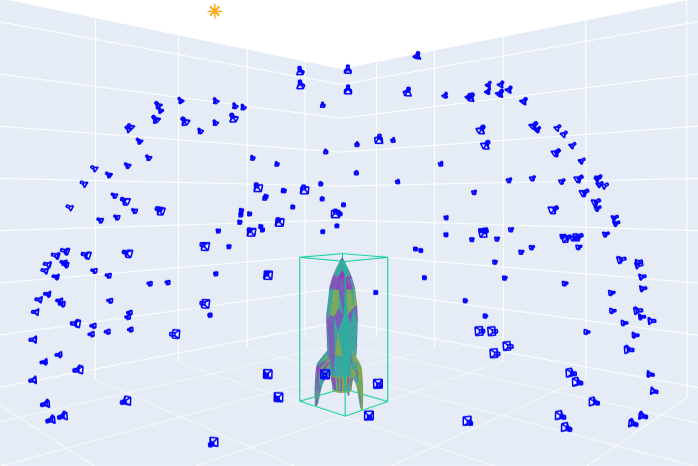
\includegraphics[width=0.32\textwidth]{figures/light_settings/static_setting.png}
        & 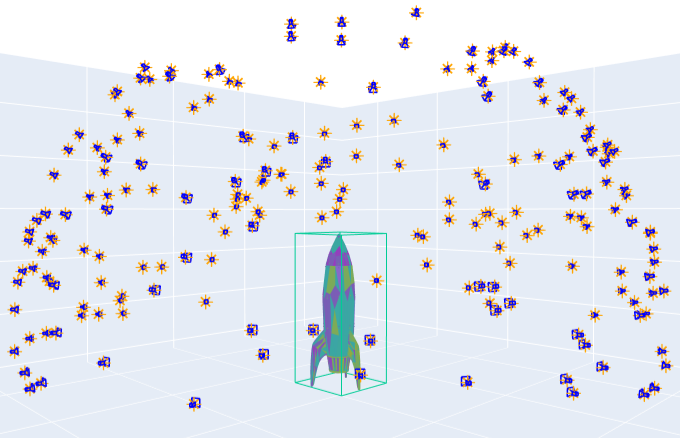
\includegraphics[width=0.29\textwidth]{figures/light_settings/colocated_setting.png}
        & 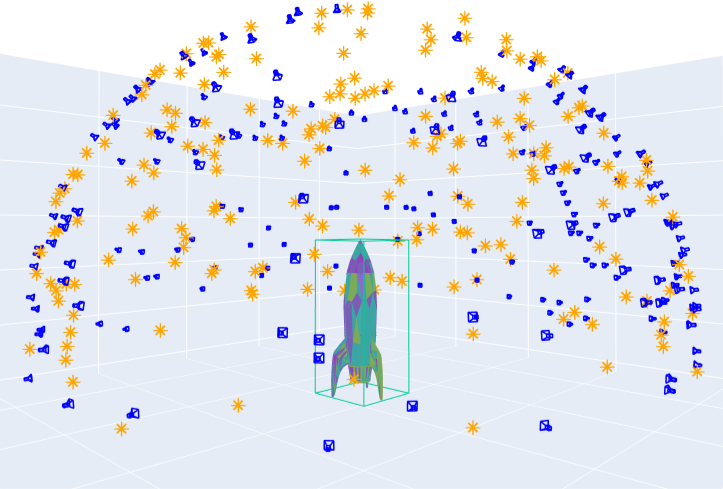
\includegraphics[width=0.29\textwidth]{figures/light_settings/arbitrary_setting.png} \\
        (a) Static & (b) Colocated & (c) Arbitrary
    \end{tabular*}
    \caption{Types of datasets that are used in the experiments.
    Cameras are denoted with blue icons, point light sources are represented by yellow stars.
    In static light setting (a) light source in all of created sample images are placed at the same point
    while camera locations are spread on a clipped sphere around the scene.
    Colocated light setting (b) imply point light sources to be placed at the same position with the camera for each sample view.
    In arbitrary light setting (c) both point light source and camera locations are spread on a clipped spheres around the scene.}
    \label{fig:light_settings}
\end{figure}
\endgroup





\subsection{Scenes}

Creating the datasets from scratch is motivated by the fact that
vast majority of related works do not consider any light interaction.
This results in such a problem that the datasets that have been used in these works
do not include any necessary light information (global position).
Another limitation of these datasets is that the light source is static upon the dataset samples,
which results in a sparse light-view sampling of the scene.
To the date of writing this thesis the datasets from correponding related works \cite{nerv2021}
still are not publicly available.
Four different scenes have been used for the evaluation (\Cref{fig:dataset_preview}).


% \CatchFileDef{\catchdatasetpreview}{tex/objects/figure_dataset_preview.tex}{}
% \catchdatasetpreview
\begingroup
\setlength{\tabcolsep}{15pt} % Default value: 6pt
\begin{figure}[!htb]
    \centering
    \begin{tabular}{cccc}
        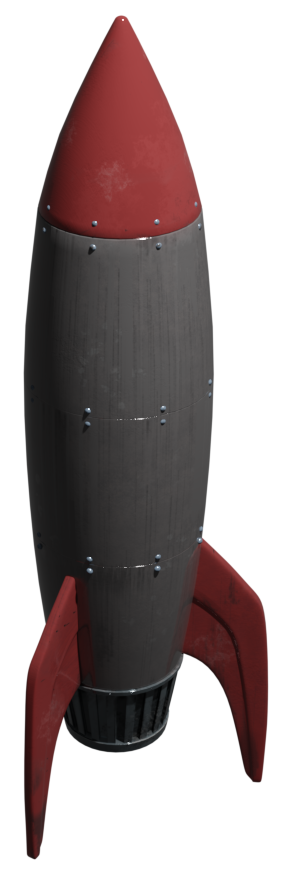
\includegraphics[width=0.1\textwidth]{figures/rocket.png}
        & 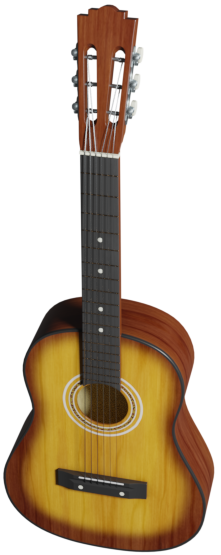
\includegraphics[width=0.13\textwidth]{figures/guitar.png}
        & 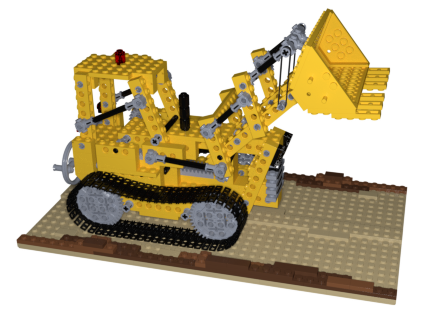
\includegraphics[width=0.30\textwidth]{figures/lego.png}
        & 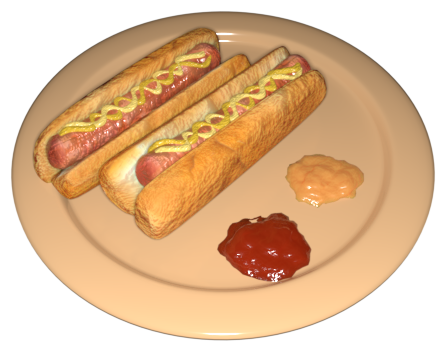
\includegraphics[width=0.25\textwidth]{figures/hotdog.png} \\
        (a) Rocket & (b) Guitar & (c) Lego & (d) Hotdog
    \end{tabular}
    \caption{
    Preview samples of the created datasets.
    All the datasets are created from the very beginning.
    (a) \cite{boucher2019rocket} and (b) \cite{legalov2020guitar} are created from publicly available 3D models in Blender \cite{blender}.
    (c) and (d) are created from 3D models that are publicly available withing NeRF work \cite{mildenhall2019local}.
}
\label{fig:dataset_preview}
\end{figure}
\endgroup

% \textbf{Sphere}

% The \textit{sphere} scene consists solely of a sphere,
% which shares Lambertian reflectance (\cite{blinn1982light}) with some specular and roughness components.
% This scene is mostly used as a baseline as it is a very simple
% both geometrically and in terms of appearance.

\textbf{Rocket}

The \textit{rocket} scene (\Cref{fig:dataset_preview} (a)) contains a single object,
which exhibits geometry of medium complexity and realistic non-Lambertian materials.
This scene contains global geometry complications (rocket wings) and some fine details (rivets on the rocket shell).
The surface of the rocket shows moderate level of specularities (in comparison with sphere scene)

\textbf{Guitar}

The \textit{guitar} scene (\Cref{fig:dataset_preview} (b)) is created for testing models ability
to reproduce highly specular surface behavior.
Complex geometry also allows to asses how model handles geometrical features on different scales.
For example strings can be barely seen on renders and they would presumably the most troublesome geometrical part of the whole scene.

\textbf{Lego}

\textit{Lego} scene (\Cref{fig:dataset_preview} (c)) is the reproduction of the model
that have been used in a former NeRF work \cite{mildenhall2020nerf}.
The dataset is recreated under a specific illumination,
which consists of only one point light source.
The object exhibits a very complex geometry on all scales.
The appearance of the surface does not show any complications.

\textbf{Hotdog}

\textit{Hotdog} scene (\Cref{fig:dataset_preview} (d)) is also a reproduction of the model
from the NeRF work with only one point light source.
The reflectance behavior of objects on this scene is more sphisticated
coparing to the \textit{lego} scene while the geometry is simpler.


\subsection{Real-world dataset handling}

For the group of methods that only consider static illumination of the scene
the dataset acquisition can be performed in different ways.
One of these ways is to use a cell phone with its camera to capture the scene.
The acquired images can then be processed with such techniques as
structure-from-motion (\cite{Moulon2012, Jancosek2011, schoenberger2016structure})
in order to retrieve the camera intrinsics and extrinsics in correspondence with captured images.
Another way is to use some special hardware setups with calibrated camera positions
such as gonioreflectometers or e.g. x-rite tac7 (\cite{merzbach2017highquality}).

However, for the methods that model light interaction the light extrinsics information is lacking
when using the aforementioned techniques.
The acquisition of the dataset consisting of captures from real-world scenes
for this group of methods is a fairly hard task that cannot be performed without any hardware assistance.
Even for the 'colocated' case of the NRF method cellphones can only be used
together with the robotic arm holding the cellphone (\cite{bi2020neural}).

Another key point is the background that has to be as homogeneous as possible.
The quality of final renders are sensitive to the too complex background behind the object on the scene.

\im{Description of faulty flower dataset??}


% \begin{enumerate}
%     \item Synthetic datasets:
%     \begin{enumerate}
%         \item static/co-located/arbitrary
%         \item Blender + python
%         \item Blender point light intensity for light attenuation
%         \item Different scenes (with its features explanations: reflectance, shape, etc.)
%     \end{enumerate}
%     \item Real-world datasets: flower??? tac7
% \end{enumerate}


\section{Implementation details}

All of the proposed methods are implemented on Python
using PyTorch \cite{pytorch} and Fairseq \cite{ott2019fairseq} frameworks
for neural fields and ray casting procedure.
During training $80$ pixels are first sampled from each of $1$ or $2$ images 
forming a batch that is used for one training iteration.
These pixels are used to cast rays through the principle points of the corresponding cameras.
These rays are then intersect the octree, which is initialized with $N_0^3 = 4^3$ voxels ($4$ voxels for each axis).
These rays are then sampled on the intersection intervals with the step size $0.125$.
The following procedure differs depending on the method
and include additional light ray casting, intersecting and sampling for the 'brute-force' scheme and BRDF evaluation for the 'explicit schemes'.
Alpha compositing is performed after the color (or radiance) values are achieved.
These values are then being supervised with the ground truth values using fine-network term from loss function from the \Cref{eq:loss_func} with the beta-distribution regularizer from the \Cref{eq:beta_regularizer}:
\begin{equation}
    \mathcal{L} = \sum_{(p_0,v)\in\mathcal{B}} \norm{ C(p, v) - C^*(p, v) } + \beta(\log(\tau_c(p, v)) + \log(1 - \tau_c(p, v))),
\end{equation}
with $\beta = 10^{-3}$ that is used in the experiments.

Adam optimizer is used as an optimization algorithm for learning parameters $(\Theta, I)$ ($I$ is light intensity value).
Learning rate for the optimizer is initialized with value $10^{-4}$
and polynomially decays to value $10^{-6}$ over 100k iterations.
Refinement procedure as well as reducing ray casting step are performed on iterations 5k, 25k and 50k.
Self-pruning is performed every 5k iterations.
Tone-mapping using scaling and gamma-correction (differ depending on scene)
is performed to visualize HDR images (both inputs and outputs).

All of the experiments are held on NVIDIA GTX 1080Ti GPU with 11GB of memory.
Dataset sample images are originally created in 1024x1024px resolution
and then individually down-sampled to some lower values for each experiment to fit the GPU memory limitations.
The resolutions from 64x64px (for \textit{brute-force scheme}) up to 512x512px 
(for methods with lower memory load, such as Vanilla NSVF) are used.
The \textit{log-transform} transformation is applied at the pre-processing phase
to prepare the HDR data before it is processed by the model:
\begin{equation}
    c = \log (c^{HDR} + 1),
\end{equation}
where $c^{HDR}$ is the color value of the HDR input
and $c$ is the color value that is used for model supervision.
The inverse-log-transform is performed on the model outputs at the post-processing stage.


% \im{64x64 for 'brute force' scheme}
% \im{different schemes - different training times. approx ~12 hours}


% \im{log transform!}


% \begin{enumerate}
%     % \item Loss function: color + beta-regularizer
%     % \item Parameters: optimizer, lr, batch, coefficients, pruning/refinement iterations
%     % \item Software/Hardware setup
%     \item Time estimates
% \end{enumerate}



\section{Metrics}

For evaluation of the results the following metrics have been used:
\begin{enumerate}
    \item \textit{PSNR}$\uparrow$ \cite{hore2010image} (Peak Signal to Noise Ratio) is a traditional estimator for image comparison
    that is based on MSE and concentrated on pixel-by-pixel comparison.
    Higher value is better.
    \item \textit{SSIM}$\uparrow$ \cite{zhou2004image, nilsson2020understanding, hore2010image} (Structural Similarity Index Measure) is a perceptual metric
    that assesses image quality based on perception of the human visual system.
    Higher value is better.
    \item \textit{LPIPS}$\downarrow$ \cite{zhang2018perceptual} (Perceptual Similarity) is the metric
    that utilizes deep features of the pre-trained deep neural networks (Alex-net \cite{krizhevsky2012imagenet} in my experiments)
    to provide an evaluation that agrees well with humans' assessments.
    Lower value is better.
    \item \textit{HDRFlipLoss}$\downarrow$ \cite{theisel2021hdrflip, andersson2020flip} is the metric
    that is aimed to work with HDR images and produce better assessment comparing to other metrics
    that were originally designed to work with LDR images.
    Lower value is better.
\end{enumerate}

Additionally to the above mentioned metrics the empirical evaluations has to be made
to assess the quality of the reproduced appearance.
This can be done by evaluating the model on a given trajectory for camera and light sources.
This produces the continuous changes in the appearance and reveals all of the artefacts of the produced renders.
The usage of artificial datasets (\Cref{sec:datasets}) allows to generate the ground truth images
even for novel light and view conditions, which are not contained in training or validation datasets.
This cannot be done for real-world images, which makes the whole task of quality assessment more difficult for such datasets.
% Metrics: MSE, SSIM, FLIPLoss/HDRFlipLoss


\section{Experiments}

The diversity of used models and the corresponding applicable datasets
does not allow to well structure this section.
A shortage of some baseline results does also contribute to some difficulties in the results quality assessment.
Therefore this section is formed in the order of increasing complexity of used methods and decreasing evaluation capabilities.
The following methods are being evaluated in either event:
\begin{enumerate}
    \item Vanilla \textit{NSVF} method \cite{liu2021neural} (described in \Cref{subsec:NSVF})
    \item Explicit colocated scheme (\textit{ExCol}) \cite{bi2020neural, liu2021neural}, which is explained in details in \Cref{subsec:NRF}
    and is a lighter version of \textit{explicit brute-force scheme}
    due to reuse of viewing sample points
    \item Explicit brute-force scheme (\textit{ExBF}) (described in \Cref{sec:explicit_scheme})
    \item Explicit approximated scheme (\textit{ExVA}), which is the \textit{explicit brute-force scheme}
    that uses the in-voxel approximation from \Cref{sec:invoxel}
    \item Implicit approximated scheme (\textit{ImVA}) \im{most likely not}
\end{enumerate}


% \CatchFileDef{\catchmethodsdatasets}{tex/objects/figure_dataset_preview.tex}{}
% \catchmethodsdatasets
\begin{table*}[!htb]
    % \setArraystrech{1.5}
    \centering
    \setlength\tabcolsep{5pt}
    \begin{tabular*}{\textwidth}{ l | c c c c c }
    	\toprule
    	 & NSVF \cite{liu2021neural} & ExCol (ours) & ExBF (ours) & ExVA (ours) & ImNRF (ours) \\
        \midrule
        Static light & \checkmark & X & \checkmark & \checkmark & \checkmark \\
    	Colocated light & X & \checkmark & \checkmark & \checkmark & \checkmark \\
    	Arbitrary light & X & X & \checkmark & \checkmark & \checkmark \\
        \midrule
        Novel views & \checkmark & \checkmark & \checkmark & \checkmark & \checkmark \\
        Novel lights & X & \checkmark & \checkmark & \checkmark & \checkmark$^*$ \\
    	\bottomrule
    \end{tabular*}
    \caption{The applicability of different types of datasets to methods.
    As can be seen from the experiments section (\Cref{subsec:experiments_coloc}),
    \textit{ImNRF's} ability for view synthesis under novel light conditions
    is highly sensitive to the type of training dataset.
    }
    \label{tab:methods_datasets}
\end{table*}

\Cref{tab:methods_datasets} shows the applicability of different types of datasets to methods that are used in experiments.






\subsection{Colocated light setting}
\label{subsec:experiments_coloc}

Datasets with the colocated light setting can be evaluated by all of the listed models except \textit{NSVF}.
The fact that a very fast \textit{ExCol} scheme can be evaluated on these datasets
makes them very advantageous for comparing against other methods.
Since the \textit{ExCol} scheme is essentially a special case for \textit{ExBF} scheme
they perform the same way as long as the sampling for light rays is performed the same way as for view rays.
In contrary, the performance of \textit{ExBF} scheme is drastically worse comparing to \textit{ExCol} scheme.
Hence the main focus here is to compare colocated scheme with the in-voxel approximation scheme.



% \CatchFileDef{\catchcolocmetrics}{tex/objects/coloc_metrics.tex}{}
% \catchcolocmetrics
\begingroup
\begin{table*}[!htb]
    % \setArraystrech{1.5}
    \centering
    \begin{tabular*}{\textwidth}{ l | l | c c c c | c c c }
        Dataset & Method & PSNR$\uparrow$ & SSIM$\uparrow$ & LPIPS$\downarrow$ & HDRFlip$\downarrow$ & Iters. & Res. & Time \\
        \midrule
        
        \multirow{4}{*}{Rocket}
        % & ExCol & 28.98 & 0.95 & 0.071 & 0.047 & 150k & 256px & 10h \\
        & ExCol & 27.69 & 0.94 & 0.088 & 0.053 & 50k & 256px & 2h30m \\
        % & ExVA & 30.52 & 0.950 & 0.061 & 0.050 & 150k & 256px & 14h \\
        & ExVA & 29.14 & 0.94 & 0.083 & 0.058 & 50k & 256px & 3h \\
        & ImNRF & \textbf{29.87} & \textbf{0.95} & \textbf{0.061} & \textbf{0.049} & 50k & 256px & 2h \\
        & \color{gray}ExBF & \color{gray}26.80 & \color{gray}0.94 & \color{gray}0.030 & 0.\color{gray}090 & \color{gray}50k & \color{gray}64px & \color{gray}6h30m \\
        \midrule
        
        \multirow{4}{*}{Guitar}
        & ExCol & 29.40 & 0.96 & 0.042 & 0.057 & 150k & 256px & 10h30m \\
        & ExVA & 29.22 & 0.96 & 0.043 & 0.059 & 150k & 256px & 20h \\
        & ImNRF & \textbf{32.56} & \textbf{0.98} & \textbf{0.017} & \textbf{0.042} & 150k & 256px & \color{bronze}20h' \\
        & \color{gray}ExBF & \color{gray}25.28 & \color{gray}0.93 & \color{gray}0.030 & \color{gray}0.120 & \color{gray}30k & \color{gray}64px & \color{gray}8h \\
        \midrule
        
        \multirow{4}{*}{Lego}
        % & ExCol & 27.02 & 0.93 & 0.07  & 0.10 & 150k & 256px & 13h \\
        & ExCol & 25.57 & 0.91 & 0.090 & 0.110 & 50k & 256px & 3h \\
        & ExVA & 25.95 & 0.92 & 0.090 & 0.110 & 50k & 256px & 4h30m \\
        & ImNRF & \textbf{26.99} & \textbf{0.93} & \textbf{0.066} & \textbf{0.099} & 50k & 256px & 2h30m \\
        & \color{gray}ExBF & \color{gray}20.76 & \color{gray}0.85 & \color{gray}0.053 & \color{gray}0.179 & \color{gray}50k & \color{gray}64px & \color{gray}6h \\
        \midrule
        
        \multirow{4}{*}{Hotdog}
        & ExCol & 32.80 & 0.96 & 0.040 & 0.075 & 70k & 256px & 6h \\
        & ExVA & 32.57 & 0.96 & 0.040 & \textbf{0.073} & 70k & 256px & \color{gray}25h$^*$ \\
        & ImNRF & \textbf{33.90} & \textbf{0.97} & \textbf{0.026} & 0.089 & 70k & 256px & \color{bronze}11h' \\
        & \color{gray}ExBF & \color{gray}24.68 & \color{gray}0.88 & \color{gray}0.059 & \color{gray}0.150 & \color{gray}70k & \color{gray}64px & \color{gray}16h \\
    \end{tabular*}
    \caption{Quantitative comparison of evaluations on colocated datasets (25\% of the whole dataset or 50 sample views).
    \textit{ExBF} scheme is only trained on 64px images due to hardware limitations
    while other methods proceed with 256px images
    (except \textit{ImNRF} on rocket dataset, which metrics are given for reference only).
    Time consumption involves training time as well as regular validation time (performed every 1k iterations).
    Reported {\color{bronze}time'} for \textit{ImNRF} method is generally non-demonstrative
    due to the unreasonable usage of too low chunking rates, which led to unrealized potential.
    \textit{ExCol} and \textit{ExVA} schemes generally produce very close results,
    although \textit{ExVA} is an approximation of the general case of \textit{ExCol} method.
    The overhead of additional calculations of \textit{ExVA} results in more time consumption.
    \textit{ImNRF} stands out from other methods by achieving better results.
    % Although the 'brute-force scheme usually takes 2-3 times more time
    % for training on 4 times smaller inputs (64px instead of 256px).
    Time measurement for \textit{ExVA} method on Hotdog dataset is not plausible
    due to adjacent circumstances limiting the hardware performance for this experiment.
    % \im{REVIEW ImNRF: waiting for results from guitar (u4103) and hotdog (u4108) in 256px}
    }
    \label{tab:colocated_metrics}
\end{table*}
\endgroup


% ExCol/Guitar/256:   u4101 -> guitar_coloc_exr
%       150k:   29.40 & 0.96 & 0.042 & 0.057 & 150k & 256px & 10h30m
%       125k:   29.38 & 0.96 & 0.042 & 0.057 & 125k & 256px & 8h30m
%       30k:    26.26 & 0.93 & 0.1 & 0.095 & 30k & 256px & 1h
% ExVA/Guitar/256:  u4102 -> guitar_coloc_exr
%       150k:   29.22 & 0.96 & 0.043 & 0.059 & 150k & 256px & 20h
%       125k:   29.22 & 0.96 & 0.044 & 0.061 & 125k & 256px & 16h
%       30k:    26.12 & 0.93 & 0.10 & 0.099 & 30k & 256px & 1h30m
% ExVA/Rocket/256:  u4103 -> rocket_coloc_exr
%       150k:   30.52 & 0.95 & 0.061 & 0.05 & 150k & 256px & 14h
%       50k:    29.14 & 0.94 & 0.083 & 0.058 & 50k & 256px & 3h
% ExCol/Rocket/256:   u4104 -> rocket_coloc_exr
%       150k:   28.98 & 0.95 & 0.071 & 0.047 & 150k & 256px & 10h
%       50k:    27.69 & 0.936 & 0.088 & 0.053 & 50k & 256px & 2h30m
% ExCol/Lego/256:     u4105 -> lego_coloc_exr
%       150k:   27.06 & 0.93 & 0.07 & 0.1 & 150k & 256px & 13h
%       125k:   27.02 & 0.93 & 0.07 & 0.1 & 125k & 256px & 11h
%       50k:    25.57 & 0.91 & 0.09 & 0.11 & 50k & 256px & 3h
% ExVA/Lego/256:    u4106 -> lego_coloc_exr
%       50k:    25.95 & 0.92 & 0.09 & 0.11 & 50k & 256px & 4h30m
% ExBF/Lego/64:     <redo>u4107 -> lego_coloc_exr
%       100k:   21.70 & 0.88 & 0.040 & 0.164 & 100k & 64px & 18h30m
%       50k:   20.76 & 0.85 & 0.053 & 0.179 & 50k & 64px & 6h
% <1st run>50k:    20.54 & 0.85 & 0.05 & 0.18 & 50k & 64px & -
% ExBF/Rocket/64:   u4108 -> rocket_coloc_exr
%       50k:    26.8 & 0.94 & 0.03 & 0.09 & 50k & 64px & 6h30m
% ExBF/Guitar/64:   u4109 -> guitar_coloc_exr
%       30k:    25.28 & 0.93 & 0.03 & 0.12 & 30k & 64px & 8h


% ExCol/Hotdog/256:   u4101 -> hotdog_coloc_exr
%       150k:   33.12 & 0.96 & 0.038 & 0.073 & 150k & 256px & 17h
%       70k:    32.80 & 0.96 & 0.04 & 0.075 & 70k & 256px & 6h
% ExVA/Hotdog/256:   u4102 -> hotdog_coloc_exr
%       150k:    &  &  &  & 150k & 256px & 
%       66k:    32.57 & 0.96 & 0.040 & 0.073 & 70k & 256px & 25h
% ExBF/Hotdog/64:   u4103 -> hotdog_coloc_exr
%       68k:    24.68 & 0.88 & 0.059 & 0.15 & 70k & 64px & 16h


% ImNRF/Rocket/256:   u4101 -> rocket_coloc_exr
% 150k ~ 
%       50k:    29.87 & 0.947 & 0.061 & 0.049 & 50k & 256px & 2h
% ImNRF/Guitar/256:   u4103 -> guitar_coloc_exr
%       150k:   32.56 & 0.98 & 0.017 & 0.042 & 150k & 256px & 20h
% ImNRF/Lego/256:   u4106 -> lego_coloc_exr
% 150k ~ ?
%       57k:   27.63 & 0.94 & 0.057 & 0.098 & 57k & 256px & 6h30m (from inefficient chunk rates)
%       50k:   26.99 & 0.93 & 0.066 & 0.099 & 50k & 256px & 2.30h
% ImNRF/Hotdog/256:   u4108 -> hotdog_coloc_exr
% 150k ~ 
%       110k:   34.81 & 0.98 & 0.021 & 0.083 & 110k & 256px & 20h30m
%       70k:    33.90 & 0.97 & 0.026 & 0.089 & 70k & 256px & 11h


        % ImNRF/Rocket/128:   u4102 -> rocket_coloc_exr
        % 150k ~ 9h30m
        %       129k:   33.83 & 0.98 & 0.015 & 0.045 & 130k & 128px & 8h
        %       50k:    30.535 & 0.966 & 0.033 & 0.055 & 50k & 128px & 2h
        % ImNRF/Guitar/128:   u4104 -> guitar_coloc_exr
        % 150k ~ 11h30m
        %       111k:   30.32 & 0.97 & 0.018 & 0.059 & 111k & 128px & 8h
        % ImNRF/Hotdog/128:   u4108 -> hotdog_coloc_exr
        % 150k ~ 
        %       88k:   33.33 & 0.98 & 0.012 & 0.099 & 88k & 128px & 8h
        %       70k:   32.87 & 0.97 & 0.013 & 0.102 & 70k & 128px & 6h30m

\Cref{tab:colocated_metrics} gives an overview of quantitative results of evaluation methods on colocated datasets.
Four aforementioned metrics are calculated on renders over the validation dataset.
The \textit{ExCol} scheme is the fastest among specified methods,
since it does not evaluate any overhead related to sampling light rays
as the view samples are simply reused as samples for light rays.
The \textit{ExVA} scheme is an approximation of \textit{ExCol} method
that uses the distance of travel of light rays inside the voxels scaled by some constant sigma value.
The implementation implies light rays intersection with the octree,
which is a fairly fast task, although it still substantially drops the performance.
The approximation scheme \textit{ExVA} is from $1.4$ to $2$ times slower
than the fastest \textit{ExCol} depending on the scene.
% The best values are denoted in bold.
The \textit{ExCol} scheme does produce mostly better results,
which should be similar to \textit{ExBF} method.
However, the \textit{ExBF} method has a massive overhead in sampling light rays
and evaluating model on these samples,
which makes it naturally impractical.
Training of \textit{ExBF} model even on 64px images takes $1.5$ times more time
than training approximation \textit{ExVA} scheme on 256px images.
In these experiments the \textit{ExBF} scheme did not manage
to converge completely due to the hardware memory limitations.
Interestingly the \textit{ExBF} method performed better according to
LPIPS metric, even though it did not converge completely.
This could be the result of same nature of the LPIPS metric
that uses deep features for the evaluation.
Some outputs of these experiments are selected from the validation dataset
and overviewed in \Cref{tab:coloc_allresults}.
% \textit{ExCol} and \textit{ExVA} methods have been trained using 256x256px images
% while the brute-force scheme \textit{ExBF} was only trained using 64x64px images.
% The reason for that is a huge need of the \textit{ExBF} method for memory,
% which is limited by the hardware.
The refinement procedure is performed on 5k, 25k and 50k iterations.
For the \textit{ExBF} method the third refinement procedure requires too much memory,
so the training only consists of 50k iterations.


\begingroup
\begin{table*}[!htb]
    % \setArraystrech{1.5}
    \centering
    \caption{\im{Fix width and add description!}}
    \label{tab:coloc_setting_imgs}
    \begin{tabular*}{\textwidth}{ c c c c }
        Target (256px) & ExCol (256px) & ExVA (256px) & ExBF (64px) \\
        %%%%% GUITARS %%%%%
        \setlength\tabcolsep{0pt}
        \begin{tabular}{cc}
            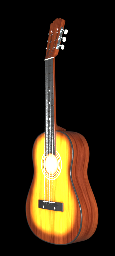
\includegraphics[width=0.1\textwidth]{figures/results/col_set/guitar0_targ_256px.png} & 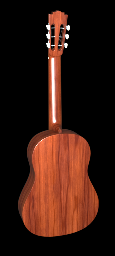
\includegraphics[width=0.1\textwidth]{figures/results/col_set/guitar8_targ_256px.png}
        \end{tabular}
        &
        \setlength\tabcolsep{0pt}
        \begin{tabular}{cc}
            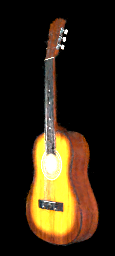
\includegraphics[width=0.1\textwidth]{figures/results/col_set/guitar0_excol_150k.png} & 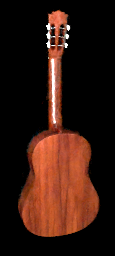
\includegraphics[width=0.1\textwidth]{figures/results/col_set/guitar8_excol_150k.png}
        \end{tabular}
        &
        \setlength\tabcolsep{0pt}
        \begin{tabular}{cc}
            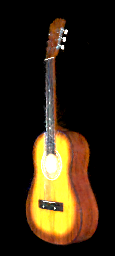
\includegraphics[width=0.1\textwidth]{figures/results/col_set/guitar0_exva_132k.png} & 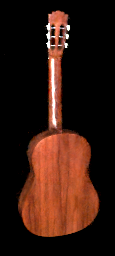
\includegraphics[width=0.1\textwidth]{figures/results/col_set/guitar8_exva_132k.png}
        \end{tabular}
        &
        \setlength\tabcolsep{0pt}
        \begin{tabular}{cc}
            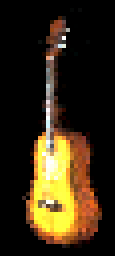
\includegraphics[width=0.1\textwidth]{figures/results/col_set/guitar0_exbf_32k.png} & 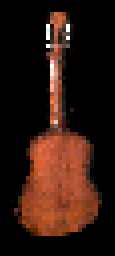
\includegraphics[width=0.1\textwidth]{figures/results/col_set/guitar8_exbf_32k.png}
        \end{tabular} \\[-5pt]
        & 150k & 125k & 30k \\
        
        
        %%%%% ROCKET %%%%%
        \setlength\tabcolsep{0pt}
        \begin{tabular}{cc}
            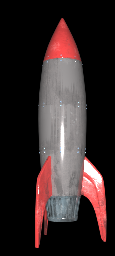
\includegraphics[width=0.1\textwidth]{figures/results/col_set/rocket0_targ_256px.png} & 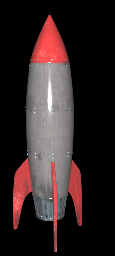
\includegraphics[width=0.1\textwidth]{figures/results/col_set/rocket4_targ_256px.png}
        \end{tabular}
        &
        \setlength\tabcolsep{0pt}
        \begin{tabular}{cc}
            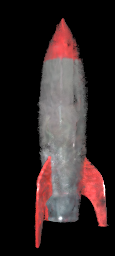
\includegraphics[width=0.1\textwidth]{figures/results/col_set/rocket0_excol_150k.png} & 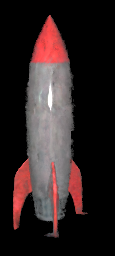
\includegraphics[width=0.1\textwidth]{figures/results/col_set/rocket4_excol_150k.png}
        \end{tabular}
        &
        \setlength\tabcolsep{0pt}
        \begin{tabular}{cc}
            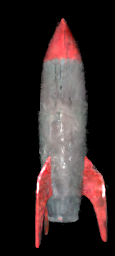
\includegraphics[width=0.1\textwidth]{figures/results/col_set/rocket0_exva_150k.png} & 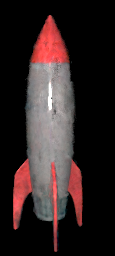
\includegraphics[width=0.1\textwidth]{figures/results/col_set/rocket4_exva_150k.png}
        \end{tabular}
        &
        \setlength\tabcolsep{0pt}
        \begin{tabular}{cc}
            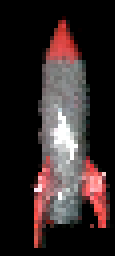
\includegraphics[width=0.1\textwidth]{figures/results/col_set/rocket0_exbf_52k.png} & 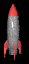
\includegraphics[width=0.1\textwidth]{figures/results/col_set/rocket4_exbf_52k.png}
        \end{tabular} \\[-5pt]
        & 150k & 150k & 50k \\
        
        %%%%% LEGO1 %%%%%
        \begin{tabular}{cc}
            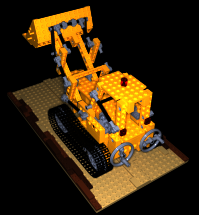
\includegraphics[width=0.2\textwidth]{figures/results/col_set/lego9_targ_256px.png} \\[-6pt]
            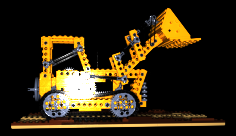
\includegraphics[width=0.2\textwidth]{figures/results/col_set/lego1_targ_256px.png}
        \end{tabular}
        &
        \begin{tabular}{cc}
            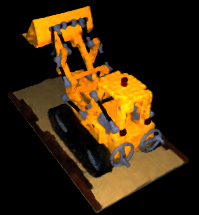
\includegraphics[width=0.2\textwidth]{figures/results/col_set/lego9_excol_57k.png} \\[-6pt]
            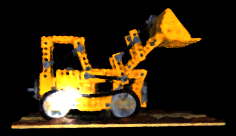
\includegraphics[width=0.2\textwidth]{figures/results/col_set/lego1_excol_57k.png}
        \end{tabular}
        &
        \begin{tabular}{cc}
            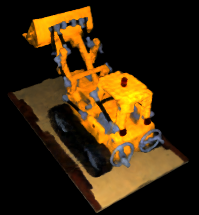
\includegraphics[width=0.2\textwidth]{figures/results/col_set/lego9_exva_51k.png} \\[-6pt]
            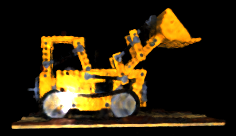
\includegraphics[width=0.2\textwidth]{figures/results/col_set/lego1_exva_51k.png}
        \end{tabular}
        &
        \begin{tabular}{cc}
            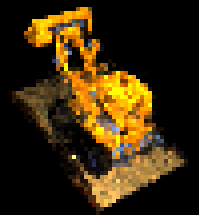
\includegraphics[width=0.2\textwidth]{figures/results/col_set/lego9_exbf_62k_voxeldefect.png} \\[-6pt]
            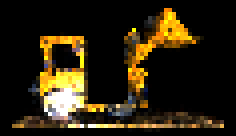
\includegraphics[width=0.2\textwidth]{figures/results/col_set/lego1_exbf_62k_voxeldefect.png}
        \end{tabular} \\[-5pt]
        & 60k & 50k & 50k \\
        
        %%%%% HOTDOG %%%%%
        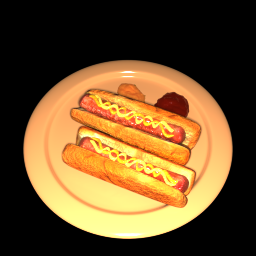
\includegraphics[width=0.2\textwidth]{figures/results/col_set/hotdog_targ_256px.png}
        &
        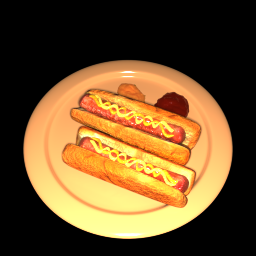
\includegraphics[width=0.2\textwidth]{figures/results/col_set/hotdog_targ_256px.png}
        &
        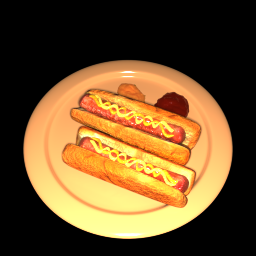
\includegraphics[width=0.2\textwidth]{figures/results/col_set/hotdog_targ_256px.png}
        &
        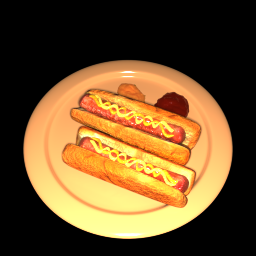
\includegraphics[width=0.2\textwidth]{figures/results/col_set/hotdog_targ_256px.png}
        \\ [-5pt]
        & \im{targ} & \im{targ} & \im{targ} \\
        

    \end{tabular*}
\end{table*}
\endgroup

Some selected views from these experiments are presented for the comparison in \Cref{tab:coloc_allresults}.
The \textit{ExBF} results are originally in 64px resolution and scaled up for clearer comparison.
The main focus is to compare results of \textit{ExCol} and \textit{ExVA} schemes.
The approximation scheme seems to produce results on the same level of quality as the colocated method.
Both schemes are occasionally lacking specularities (rocket left)
and fail reproducing very fine details of the Lego dataset.
However, this can be the result of underfitting of this exact experiment.



\subsubsection{ExCol vs. NRF}

The \textit{ExCol} scheme is originally based on NRF framework \cite{bi2020neural},
which extends the problem of novel view rendering to
'novel view-light rendering' by considering reflectance of the objects in the scene.
However, \textit{ExCol} method in turn uses NSVF framework for increasing the efficiency of sampling.
Although \cite{bi2020neural} do not provide the datasets from their experiments,
some rough time estimation comparison can be done.
It takes approximately 48 hours for the NRF model to get trained on 4 GPUs NVIDIA RTX 2080Ti.
This hardware setup is much more powerful than the hardware used in this thesis.
Nevertheless as it can be seen from \Cref{tab:colocated_metrics}
the \textit{ExCol} can get trained in approximately 12 hours on a single GPU NVIDIA 1080Ti,
which is $4$ times faster than original NRF approach.
Even considering the differences in the datasets and quantitative differences in achieved results,
the efficiency improvement is fairly distinct.
Unfortunately, \cite{bi2020neural} do not provide any metrics values to compare our results with.




\subsection{Arbitrary light setting}

Datasets with the arbitrary setting can only be processed with 
brute-force \textit{ExBF} and voxel-approximation \textit{ExVA} schemes
since the light source is not co-located with the camera,
which is the requirement for the \textit{ExCol} scheme.
The \textit{ExBF} method is an impractically slow generalization for the \textit{ExCol}.
Thus the \textit{ExVA} is the main method for achieving renders on this type of datasets.
Although \textit{ExVA} is an approximation,
which theoretically produces worse results than the 'brute-force' or 'colocated' schemes,
experiments with the colocated datasets (\Cref{subsec:experiments_coloc}) showed
that evaluations are very similar between \textit{ExVA} and \textit{ExCol}
by assessing both using metrics (\Cref{tab:colocated_metrics}) or empirically (\Cref{tab:coloc_allresults}).

\Cref{tab:arb_selective_results} gives an overview on the results of two mentioned above methods
trained on Lego dataset with an arbitrary light setting.
Images labeled with \textit{HDRFlip} are the difference images produced within HDRFlipLoss \cite{andersson2020flip, theisel2021hdrflip}
between target images and corresponding renders.
The \textit{ExBF} method is again trained only on 64px images due to hardware limitations.
The down-sampled version of target image is used to calculate HDRFlip image for \textit{ExBF}.
It can be seen that the model did reproduce the scene with fairly high quality,
although it produces more errors on darker views with some highly specular flares (3rd line of images in table).
Please note that images on the 3rd line are post-processed by scaling and applying gamma-correction ($\gamma = 2.5$)
and in reality they contain very dark object with a very bright spot of light reflection.


\subsubsection{Novel light synthesis}

Although \cite{bi2020neural} claim that deep neural network from their framework
can generalize to some arbitrary light position while only being trained on coinciding light-view positions,
the quality of this generalization is still doubtful.
Datasets that were created with the arbitrary light setting
contain denser light-view sample space than those created with colocated setting.
This results in a higher quality of novel-light synthesized views.
\Cref{tab:arb_dynamic_light} contains five images, evaluated from the same novel (has not been used during training) camera position.
Each of these images is lit from the light source that is located at the novel light position.
Light rays to the center of the scene form with a view ray to the center of scene angles
that are denoted under each column of images.
It can be clearly seen that \textit{ExVA} method outperforms \textit{ExCol}.
The major difference is in the capability of rendering shadows (non-zero angles)
while for the zero-angle view both methods perform with approximately the same quality.
Please note that for this experiment \textit{ExCol} has been trained on the dataset with colocated light setting
whilst \textit{ExVA} has been trained on the dataset with arbitrary light setting.




% ExVA/Lego/256:     u4108 -> lego_random_exr
%       150k:   24.00 & 0.88 & 0.101 & 0.207 & 150k & 256px & 11h30m
%       80k:    23.76 & 0.87 & 0.117 & 0.215 & 80k & 256px & 5h

\begingroup
\begin{figure}[!htb]
    % \setArraystrech{1.5}
    \centering
    \setlength\tabcolsep{2pt}
    \begin{tabular*}{\textwidth}{ c c c c c }
        HDRFlip$_{ExVA}$ & ExVA & Target & ExBF & HDRFlip$_{ExBF}$ \\
        % \multicolumn{2}{c}{256px} & 256px & \multicolumn{2}{c}{64px} \\
        256px & 256px & 256px & 64px & 64px \\
        
          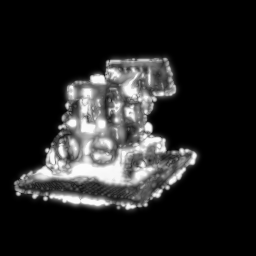
\includegraphics[width=0.19\textwidth]{figures/results/arb_set/validation/lego6_exva_hdrflip_150k.png}
        & 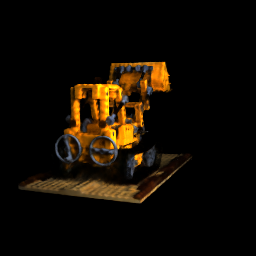
\includegraphics[width=0.19\textwidth]{figures/results/arb_set/validation/lego6_exva_150k.png}
        & 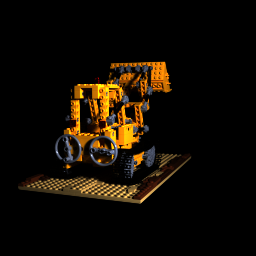
\includegraphics[width=0.19\textwidth]{figures/results/arb_set/validation/lego6_targ_256px.png}
        & 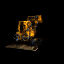
\includegraphics[width=0.19\textwidth]{figures/results/arb_set/validation/lego6_exbf_112k.png}
        & 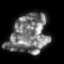
\includegraphics[width=0.19\textwidth]{figures/results/arb_set/validation/lego6_exbf_hdrflip_112k.png} \\[-6pt]
        
          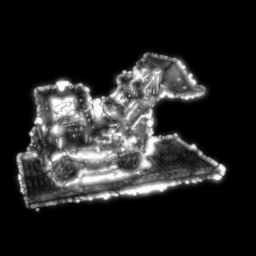
\includegraphics[width=0.19\textwidth]{figures/results/arb_set/validation/lego7_exva_hdrflip_150k.png}
        & 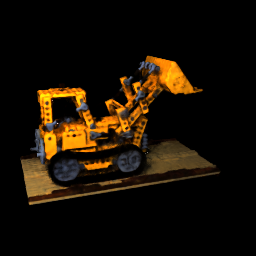
\includegraphics[width=0.19\textwidth]{figures/results/arb_set/validation/lego7_exva_150k.png}
        & 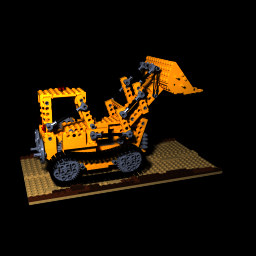
\includegraphics[width=0.19\textwidth]{figures/results/arb_set/validation/lego7_targ_256px.png}
        & 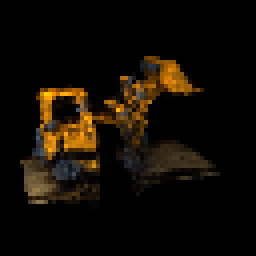
\includegraphics[width=0.19\textwidth]{figures/results/arb_set/validation/lego7_exbf_112k.png}
        & 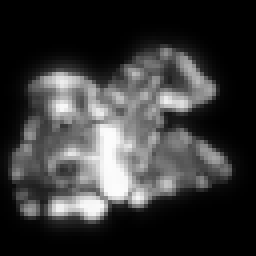
\includegraphics[width=0.19\textwidth]{figures/results/arb_set/validation/lego7_exbf_hdrflip_112k.png} \\[-6pt]
        
          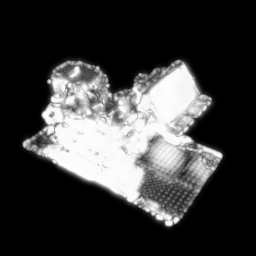
\includegraphics[width=0.19\textwidth]{figures/results/arb_set/validation/lego10_exva_hdrflip_150k.png}
        & 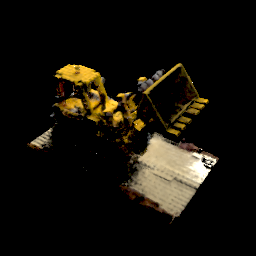
\includegraphics[width=0.19\textwidth]{figures/results/arb_set/validation/lego10_exva_150k.png}
        & 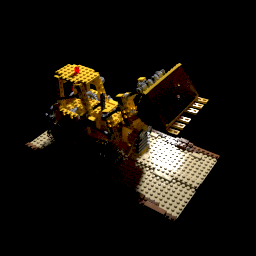
\includegraphics[width=0.19\textwidth]{figures/results/arb_set/validation/lego10_targ_256px.png}
        & 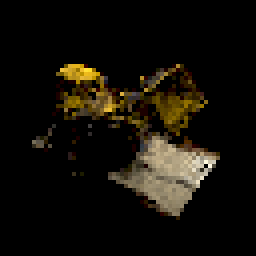
\includegraphics[width=0.19\textwidth]{figures/results/arb_set/validation/lego10_exbf_112k.png}
        & 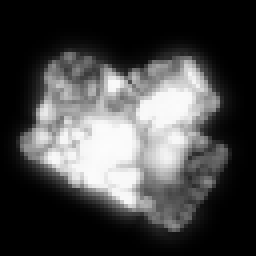
\includegraphics[width=0.19\textwidth]{figures/results/arb_set/validation/lego10_exbf_hdrflip_112k.png} \\[-6pt]
        
          \includegraphics[width=0.19\textwidth]{figures/results/arb_set/validation/lego14_exva_hdrflip_150k.png}
        & \includegraphics[width=0.19\textwidth]{figures/results/arb_set/validation/lego14_exva_150k.png}
        & \includegraphics[width=0.19\textwidth]{figures/results/arb_set/validation/lego14_targ_256px.png}
        & \includegraphics[width=0.19\textwidth]{figures/results/arb_set/validation/lego14_exbf_112k.png}
        & \includegraphics[width=0.19\textwidth]{figures/results/arb_set/validation/lego14_exbf_hdrflip_112k.png}
        

    \end{tabular*}
    \caption{The overview of some novel light-view synthesis results
    achieved with our methods trained on arbitrary light setting Lego dataset for 100k iterations.
    Rows correspond to one specific light-view location.
    Central column contains target images,
    synthesized images are on the sides from central column.
    First and last columns contain difference images
    calculated between corresponding predictions and target images using HDRFlipLoss (\Cref{sec:metrics}).
    256px images have been used for \textit{ExVA} scheme,
    while \textit{ExBF} method only used 64px images due to hardware limitations.
    Renders from the third row have been post-processed (gamma-correction with $\gamma = 2.5$ and scaling)
    since the original view is very dark with very bright spot from the reflection of the light source.
    \im{CHANGE ExBF to ImNF results!!!}
    }
    \label{tab:arb_selective_results}
\end{figure}
\endgroup

% % % ExVA/Lego/256:     u4108 -> lego_random_exr
% %       150k:   24.00 & 0.88 & 0.101 & 0.207 & 150k & 256px & 11h30m
% %       80k:    23.76 & 0.87 & 0.117 & 0.215 & 80k & 256px & 5h

% \begingroup
% \begin{table*}[!htb]
%     % \setArraystrech{1.5}
%     \centering
%     \setlength\tabcolsep{2pt}
%     \begin{tabular*}{\textwidth}{ c c c c }
%           \includegraphics[width=0.19\textwidth]{figures/results/arb_set/lego7_exva_150k.png}
%         & \includegraphics[width=0.19\textwidth]{figures/results/arb_set/lego7_exva_normal_150k.png}
%         & \includegraphics[width=0.19\textwidth]{figures/results/arb_set/lego7_exva_roughness_150k.png}
%         & \includegraphics[width=0.19\textwidth]{figures/results/arb_set/lego7_exva_depth_150k.png} \\
        
%           \includegraphics[width=0.19\textwidth]{figures/results/arb_set/lego7_exva_voxel_4k.png}
%         & \includegraphics[width=0.19\textwidth]{figures/results/arb_set/lego7_exva_voxel_18k.png}
%         & \includegraphics[width=0.19\textwidth]{figures/results/arb_set/lego7_exva_voxel_45k.png}
%         & \includegraphics[width=0.19\textwidth]{figures/results/arb_set/lego7_exva_voxel_150k.png}
        

%     \end{tabular*}
%     \caption{\im{Fix width and add description!}}
%     \label{tab:arb_maps}
% \end{table*}
% \endgroup

% exva_rand - ExVA on lego_random_exr (u4108) 150k
% excol_coloc - ExCol on lego_coloc_exr (u4105) 150k
% imnf_coloc - ImNRF on lego_coloc_exr (u4106) 64k
% imnf_rand - ImNRF on lego_rand_exr (u4107) 69k
\begingroup
\begin{figure}[!htb]
    % \setArraystrech{1.5}
    \centering
    \setlength\tabcolsep{0pt}
    \begin{tabular*}{\textwidth}{ c c c c c }
        \multicolumn{5}{c}{\textit{ImNRF} trained on \textbf{colocated} light dataset} \\
          \includegraphics[width=0.2\textwidth]{figures/results/arb_set/dynamic_light/imnf_coloc_vc0_ld-90.png}
        & \includegraphics[width=0.2\textwidth]{figures/results/arb_set/dynamic_light/imnf_coloc_vc0_ld-60.png}
        & \includegraphics[width=0.2\textwidth]{figures/results/arb_set/dynamic_light/imnf_coloc_vc0_ld0.png}
        & \includegraphics[width=0.2\textwidth]{figures/results/arb_set/dynamic_light/imnf_coloc_vc0_ld60.png} 
        & \includegraphics[width=0.2\textwidth]{figures/results/arb_set/dynamic_light/imnf_coloc_vc0_ld90.png} \\
        
        \multicolumn{5}{c}{\textit{ExCol} trained on \textbf{colocated} light dataset} \\
          \includegraphics[width=0.2\textwidth]{figures/results/arb_set/dynamic_light/excol_col_vc0_ld-90.png}
        & \includegraphics[width=0.2\textwidth]{figures/results/arb_set/dynamic_light/excol_col_vc0_ld-60.png}
        & \includegraphics[width=0.2\textwidth]{figures/results/arb_set/dynamic_light/excol_col_vc0_ld0.png}
        & \includegraphics[width=0.2\textwidth]{figures/results/arb_set/dynamic_light/excol_col_vc0_ld60.png} 
        & \includegraphics[width=0.2\textwidth]{figures/results/arb_set/dynamic_light/excol_col_vc0_ld90.png} \\

        \multicolumn{5}{c}{\textit{ExVA} trained on \textbf{arbitrary} light dataset} \\
          \includegraphics[width=0.2\textwidth]{figures/results/arb_set/dynamic_light/exva_rand_vc0_ld-90.png}
        & \includegraphics[width=0.2\textwidth]{figures/results/arb_set/dynamic_light/exva_rand_vc0_ld-60.png}
        & \includegraphics[width=0.2\textwidth]{figures/results/arb_set/dynamic_light/exva_rand_vc0_ld0.png}
        & \includegraphics[width=0.2\textwidth]{figures/results/arb_set/dynamic_light/exva_rand_vc0_ld60.png} 
        & \includegraphics[width=0.2\textwidth]{figures/results/arb_set/dynamic_light/exva_rand_vc0_ld90.png} \\

        \multicolumn{5}{c}{\textit{ImNRF} trained on \textbf{arbitrary} light dataset} \\
          \includegraphics[width=0.2\textwidth]{figures/results/arb_set/dynamic_light/imnf_rand_vc0_ld-90.png}
        & \includegraphics[width=0.2\textwidth]{figures/results/arb_set/dynamic_light/imnf_rand_vc0_ld-60.png}
        & \includegraphics[width=0.2\textwidth]{figures/results/arb_set/dynamic_light/imnf_rand_vc0_ld0.png}
        & \includegraphics[width=0.2\textwidth]{figures/results/arb_set/dynamic_light/imnf_rand_vc0_ld60.png} 
        & \includegraphics[width=0.2\textwidth]{figures/results/arb_set/dynamic_light/imnf_rand_vc0_ld90.png} \\
        
        \multicolumn{5}{c}{Target images} \\
          \includegraphics[width=0.2\textwidth]{figures/results/arb_set/dynamic_light/targ_vc0_ld-90.png}
        & \includegraphics[width=0.2\textwidth]{figures/results/arb_set/dynamic_light/targ_vc0_ld-60.png}
        & \includegraphics[width=0.2\textwidth]{figures/results/arb_set/dynamic_light/targ_vc0_ld0.png}
        & \includegraphics[width=0.2\textwidth]{figures/results/arb_set/dynamic_light/targ_vc0_ld60.png} 
        & \includegraphics[width=0.2\textwidth]{figures/results/arb_set/dynamic_light/targ_vc0_ld90.png} \\[-4pt]
        
        -90\textdegree & -60\textdegree & 0\textdegree & 60\textdegree & 90\textdegree
        

    \end{tabular*}
    \caption{Novel view-light synthesis results.
The \textit{ExCol} model is trained on dataset with colocated light setting
while \textit{ExVA} mode is trained on dataset with arbitrary light setting.
Both camera view as well as light source location are novel for both methods.
Camera is fixed at the same position for all of renders.
Point light source location is changing along rows:
inclination angle $\theta = \const$, azimuthal angle $\phi$ is changing from -90$^{\circ}$ to 90$^{\circ}$. On central column light source is co-located with camera.
\im{REVIEW!!! ImNRF images: imnf-coloc 64k u4106 256, imnf-rand 69k u4107 256}
}
    \label{tab:arb_dynamic_light}
\end{figure}
\endgroup


\im{RESULTS metrics+renders: check quality from u4108: exva lego 256px, timings can be compared on 64px results: exva u4104 vs exvf u4109}

\im{Random datasets: compare brute-force with in-voxel approximation}

% The experiments involve training models on different synthetic datasets (\im{reference to prev. subsection}) with different parameters
% and quantitative (\im{ref}) and qualitative (\im{ref}) comparisons of those.




\subsection{Static light setting}

Static light setting is the only type of datasets that can be used
for training the original NSVF method,
due to the limitation of the illumination to be static.
All other methods not only can process this dataset but also render the scene under novel light conditions.$\sup$

\im{Figure N} shows results ...

\im{Conclusion: static for explicit schemes is a very sparse arbitrary, so difficult to train}


\section{Discussion}

\begin{enumerate}
    \item HDR inputs: preprocessing (log-transform)
    \item Background color problem?
    -- NSVF used way bigger batch size (32 images instead of 2 in my case) and 2048 rays in each image (80 in my case)
    \item In-Voxel approximation: different sigma strategies
    \item Implicit scheme with tangential coordinate system
\end{enumerate}

\im{inference time estimates}
\im{show albedo/roughness/normals}


% \section{Colocated setting flaws}

% Network barely generalizes for noncolocated light source position when trained only on colocated setting


% \section{Brute Force vs Approximation}






% \section{Blender-Radiance coefficient}

% The light attenuation factor has to be taken into account in the explicit scheme.

% $L_o(x, \Omega_o) = L_e(x, \Omega_o) + \int_{H_i}{f_{BRDF}(\Omega_i, x, \Omega_o) L_i(x, \Omega_i) cos \Theta_i d\omega_i}$

% $L_i = \tau_l L_l$

% $L_l = f_{att}I$

% $f_{att}=\frac{1}{1 + 2d/r + d/r^2}$

% $L_o = \frac{k_d}{\pi} \frac{1}{1 + 2d/r + d/r^2} I cos \Theta_i$

% $k_c = 0, k_l = 0, k_q = 1$

% r = 0.05

% $f_{att} = r^2 / d = 0.0025 / (10-0.05) = 2.51256e-4$

% $0.24316406 = 0.8 / \pi * 2.51256e-4 * I * 1$

% $0.24316406 = 2.01005e-4 * I$

% $I = 500$





% This is some test area for new mathematical helper macros to nicely visualize mathematical formulas.

% \section{Numbers}
% \begin{align}
%     \mathbb{C}
%     \qquad
%     \mathbb{R}
%     \qquad
%     \mathbb{Q}
%     \qquad
%     \mathbb{Z}
%     \qquad
%     \mathbb{N}
% \end{align}

% \section{Numbers with physical units}
% \begin{align}
%     \SI{1.23}{\meter\per\second}
% \end{align}
% \begin{align}
%     \si{\meter\per\second}
% \end{align}
% \begin{align}
%     \SI{1.23\pm0.45}{\meter\per\second}
% \end{align}
% \begin{align}
%     \SI{3e8}{\meter\per\second}
% \end{align}
% \begin{align}
%     \SI{32}{\giga\byte} = \SI{32e9}{\byte}
% \end{align}
% \begin{align}
%     \SI{32}{\gibi\byte} = \SI[exponent-base=2]{32e30}{\byte}
% \end{align}

% \section{Norm, Dot, Abs, Interval}
% \begin{align}
%     \pi = \const
% \end{align}
% \begin{align}
%     1 \in \interval{0}{2}
% \end{align}
% \begin{align}
%     1 \in \order{n}
% \end{align}
% \begin{align}
%     \evalat{ \frac{\partial f}{\partial x} }{ x = 0 }
% \end{align}
% \begin{align}
%     \norm{p} \qquad \norm{\frac{p}{2}}
% \end{align}
% \begin{align}
%     \abs{p} \qquad \abs{\frac{p}{2}}
% \end{align}
% \begin{align}
%     \dotproduct{p}{q} \qquad \dotproduct{\frac{p}{2}}{q}
% \end{align}
% \begin{align}
%     \crossproduct{p}{q} \qquad \crossproduct{\frac{p}{2}}{q}
% \end{align}

% \section{Vector, Matrix}
% \begin{align}
%     \vec{p} \qquad \vecarrow{p}
% \end{align}
% \begin{align}
%     \vec{p}^{\transposed}
% \end{align}
% \begin{align}
%     \gradient{\vec{p}}
% \end{align}
% \begin{align}
%     \divergence{\mat{A}}
% \end{align}
% \begin{align}
%     \laplacian{\mat{A}}
% \end{align}
% \begin{align}
%     \mat{A}
% \end{align}
% \begin{align}
%     \set{K} , K
%     \qquad
%     \set{N} , N
% \end{align}
% \begin{align}
%     \neighborhood{\vec{p}} = \left\{ \vec{q} \mid \norm{\vec{p} - \vec{q}} < \epsilon \right\}
% \end{align}

% \section{Set operations}
% \begin{align}
%     A \intersect B
% \end{align}
% \begin{align}
%     A \union B
% \end{align}
% \begin{align}
%     A \difference B
% \end{align}

% \section{Derivative, Integral, Sum, Probability}
% \begin{align}
%     \int_H x \, dx
% \end{align}
% \begin{align}
%     \sum_H x
% \end{align}
% \begin{align}
%     \probability{x}
% \end{align}
% \begin{align}
%     \probabilitygiven{x}{y}
% \end{align}
% \begin{align}
%     \expectation{x}
% \end{align}
% \begin{align}
%     \deviation{x}
% \end{align}
% \begin{align}
%     \variance{x}
% \end{align}


% \section{Lemma, Theorem, Corollary}
% \begin{lemma}
%     This is a lemma.
% \end{lemma}
% \begin{proof}
%     Proof of lemma.
% \end{proof}

% \begin{theorem}
%     This is a theorem.
% \end{theorem}
% \begin{proof}
%     Proof of theorem.
% \end{proof}

% \begin{corollary}
%     This is a corollary.
% \end{corollary}
% \begin{proof}
%     Proof of corollary.
% \end{proof}